%# -*- coding: utf-8-unix -*-
%%==================================================
\chapter{使用示例}\label{ch1}

\section{各类环境的用法}\label{ch1se1}

\begin{mydef}{共轭点}{共轭点的定义}
	设~$(M,g)$~是~Riem~流形，$p\in M,\boldsymbol{v}\in T_{p}M$. 若~$\boldsymbol{v}$~是指数映射~$\operatorname{exp}_{p}$~的临界点，则称~$q=\operatorname{exp}_{p}(\boldsymbol{v})$~是点~$p$~沿着测地线~$\gamma(t)=\operatorname{exp}_{p}(t \boldsymbol{v})$~的共轭点. 它就是指数映射~$\operatorname{exp}_{p}$~的临界值.
\end{mydef}

\begin{myprop}{}{共轭点的等价定义}
	设~$\gamma:[0,l]\longrightarrow M$~为弧长参数测地线，$\gamma(0)=p$. 则~$q=\gamma(t_{0}),t_{0}\in (0,l]$~为~$p$~沿~$\gamma$~的共轭点，当且仅当~$ \boldsymbol{v}_{0}=t_{0}\gamma^{\prime}(0)$~是指数映射~$\operatorname{exp}_{p}$~的临界点.
\end{myprop}

\begin{proof}
	注意到~$\gamma(t)=\operatorname{exp}_{p}(t \gamma^{\prime}(0))$，故~$\operatorname{exp}_{p}(\boldsymbol{v}_{0})=\operatorname{exp}_{p}(t_{0}\gamma^{\prime}(0))=\gamma(t_{0})=q$. 再由\ref{def:共轭点的定义}~显然成立. 
\end{proof}

\begin{mythm}{}{共轭点是Jacobi场的零点}
	设~$\gamma:[0,l]\longrightarrow M$~为弧长参数测地线. 则~$\gamma(t_{0}),t_{0}\in (0,l]$~是~$\gamma(0)$~沿~$\gamma$~的共轭点，当且仅当存在沿~$\gamma$~的不恒为零的~Jacobi~场~$U(t)$~使得~$U(0)=\boldsymbol{0}=U(t_{0})$.
\end{mythm}

\begin{proof}
   \emph{$\Longrightarrow$} 记~$p=\gamma(0)$. 由\ref{prop:共轭点的等价定义}~知~$t_{0}\gamma^{\prime}(0)$~是指数映射~$\operatorname{exp}_{p}$~的临界点，即存在~$ \boldsymbol{w}\neq \boldsymbol{0}$~使得~$\left( \operatorname{exp}_{p} \right)_{\ast t_{0}\gamma^{\prime}(0)}(\boldsymbol{w})=\boldsymbol{0}$. 令
	\begin{equation}
		\begin{aligned}
   			U(t)\triangleq \left( \operatorname{exp}_{p} \right)_{\ast t\gamma^{\prime}(0)}(t \boldsymbol{w})
		\end{aligned}
		\label{共轭点的Jacobi场的构造}
	\end{equation}
   则~$U(t)$~沿~$\gamma$~的不恒为零的~Jacobi~场，且满足~$U(t_{0})=\boldsymbol{0}=U(0)$.
\end{proof}

\begin{remark}\label{一个注}
	若~$\operatorname{dim}(M)=n$，则沿测地线~$\gamma:[0,l]\longrightarrow M$~恰有~$n$~个线性无关的~Jacobi~场~$\{J_{1},\ldots,J_{n} \}$~满足~$J_{i}(0)=\boldsymbol{0}$. 这是因为满足~$J_{i}(0)=\boldsymbol{0}$~的~Jacobi~场~$\{J_{1},\ldots,J_{k}\}$~线性无关，当且仅当~$\{J_{1}^{\prime}(0),\ldots,J_{k}^{\prime}(0)\}$~线性无关.
\end{remark}

\begin{mypron}{}{一个有关Jacobi场的命题}
	设~$\gamma:[0,l]\longrightarrow M$~为弧长参数测地线，$\boldsymbol{v}_{1}\in T_{\gamma(0)}M,\boldsymbol{v}_{2}\in T_{\gamma(l)}M$. 若~$\gamma(l)$~不是~$\gamma(0)$~的共轭点，则存在唯一的沿~$\gamma$~的~Jacobi~场~$J(t)$~满足
   \[
      J(0)=\boldsymbol{v}_{1},J(l)=\boldsymbol{v}_{2}
   \]
\end{mypron}

\begin{mylem}{}{无共轭点则局部微分同胚}
	设~$M$~是完备~Riem~流形，$p\in M$. 若指数映射~$\operatorname{exp}_{p}:T_{p}M\longrightarrow M$~无临界点，则~$\operatorname{exp}_{p}:T_{p}M\longrightarrow M$~是局部微分同胚.
\end{mylem}

以下是一个代码环境的使用示例.

\begin{lstlisting}[language={python}, caption={图册的极大化}]
已知：拓扑流形$M$上的一个$C^{r}$图册$\Sigma$
目标：将$\Sigma$极大化

设定一个空集合$A$
for 流形$M$的每一个参数化$(U,\boldsymbol{x})$:
    if $(U,\boldsymbol{x})$与$\Sigma$中的每一个成员都$C^{r}$相容:
       将$(U,\boldsymbol{x})$存储到集合$A$中
       
最后令$\Sigma_{max}=\Sigma\bigcup A$
\end{lstlisting}

\begin{table}[!hpb]
	\centering
	\begin{tabular}{@{}llr@{}} \toprule
		特征值 & $\longleftrightarrow$ &$C^{r}$微分结构\\
		\midrule
		特征向量 & $\longleftrightarrow$ & $C^{r}$图册 \\ \bottomrule
	\end{tabular}
	\caption{$C^{r}$微分结构和$C^{r}$图册之间的关系就像特征值和特征向量之间的关系}
	\label{一个类比}
\end{table}

\begin{example}\label{第一个例子}
	设~$(M,g)$~是常(~Gauss~)曲率的~$2$~维~Riem~流形. 当~$r<\delta $~时，求测地圆~$\partial B_{r}$~的周长~$C(r)$.
	\soln 
	
	注意到若~$\{x,y\}$~为~$T_{p}M$~的直角坐标系，则~$x=\rho \cos\theta,y=\rho\sin\theta$. 于是
\end{example}

\begin{figure}[!htp]  
		\centering
		\scalebox{1}[0.9]{
		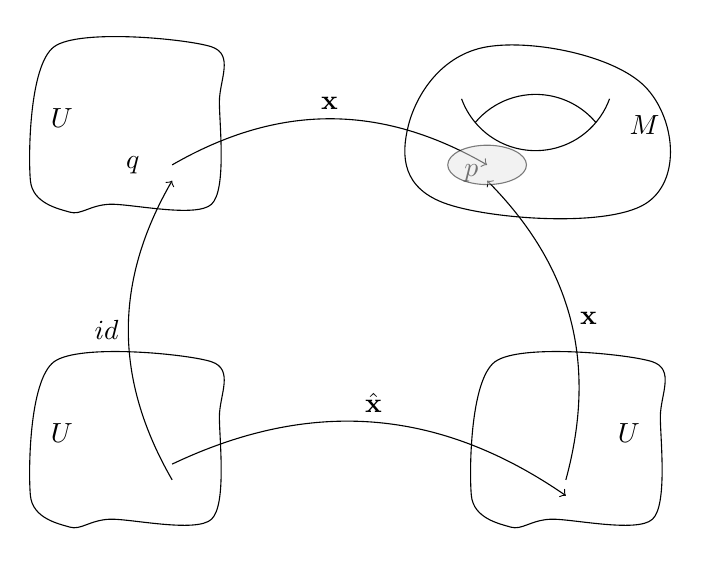
\begin{tikzpicture}
		\draw plot [smooth cycle] coordinates {(-5.3,2.4)(-4.8,2.5)(-3.5,2.5)(-3.4,3.8)(-3.5,4.5)(-5.5,4.5)(-5.8,2.8)} node at (-5.4,3.6) {$U$};
		\draw plot [smooth cycle] coordinates {(0.3,2.4)(0.8,2.5)(2.1,2.5)(2.2,3.8)(2.1,4.5)(0.1,4.5)(-0.2,2.8)} node at (1.8,3.6) {$U$};
		\draw[smooth cycle,tension=.7] plot coordinates{(-0.5,6.5) (-1,7.5) (0,8.5) (2,8) (2,6.5)};
		\coordinate (A) at (-0.1505,7.5383) {};
		\draw (A) arc (140.0041:40.0074:1) (A) arc (-139.9942:-19.9952:1) (A) arc (-140.003:-160.012:1);
		\path[->] (-4,7) edge [bend left] node[above] {$\mathbf{x}$} (0,7);
		\path[->] (-4,3) edge [bend left] node[left] {$id$} (-4,6.8);
		\path[->] (1,3) edge [bend right] node[right] {$\mathbf{x}$} (0,6.8);
		
		\draw plot [smooth cycle] coordinates {(-5.3,6.4)(-4.8,6.5)(-3.5,6.5)(-3.4,7.8)(-3.5,8.5)(-5.5,8.5)(-5.8,6.8)} node at (-5.4,7.6) {$U$};
		
		\node at (-4.5,7) {$q$};
		\node at (-0.2,6.9) {$p$};
		\node at (2,7.5) {$M$};
		\path[->] (-4,3.2) edge [bend left] node[above] {$\hat{\mathbf{x}}$} (1,2.8);
		\draw [fill= gray!20,opacity=0.5] (0,7) ellipse (0.5 and 0.25);
		\end{tikzpicture}
	}
	\caption{直接用Tikz绘制图像}
	\label{直接用Tikz绘制图像}
\end{figure}

\begin{figure}[!htp] 
		\centering
		
\includegraphics[scale=0.85]{example/m3.pdf}
		\caption{插入一个现成的图片}
		\label{插入一个现成的图片}
\end{figure}

\begin{example}[标准浸入]\label{第二个例子}
	浸入映射的原型是$R^{m}$到更高维的$R^{n}$的包含(inclusion). 其中$m<n$. 即映射\[i:R^{m}\rightarrow R^{n}\Leftrightarrow i(x_{1},x_{2},\cdots,x_{m})=(x_{1},x_{2},\cdots,x_{m},\underbrace{0,\cdots,0}_{(n-m)\text{个}0})\]
	显然$i$为光滑的浸入映射，称为标准浸入.
\end{example}

有序列表环境:
\begin{itemize} 
	\item[(1)] 若对$\forall p\in M$，切映射$(d\varphi) _ { p } : T _ { p } M \rightarrow T _ { \varphi ( p ) } N$都为单射，则称$\varphi : M \rightarrow N$为一个浸入映射(immersion).
	\item[(2)] 若对$\forall p\in M$，切映射$(d \varphi) _ { p } : T _ { p } M \rightarrow T _ { \varphi ( p ) } N$都为满射，则称$\varphi : M \rightarrow N$为一个淹没映射(submersion).
\end{itemize}

无序列表环境：
\begin{itemize}
\item 若$\varphi : M ^ { m } \rightarrow N ^ { n }$为浸入映射，则必有$\operatorname{dim}(M)=m \leqslant n=\operatorname{dim}(N)$.
\item 若$\varphi : M ^ { m } \rightarrow N ^ { n }$为淹没映射，则必有$\operatorname{dim}(M)=m \geqslant n=\operatorname{dim}(N)$.
\end{itemize}

\subsection{交叉引用}\label{ch1subse1}

本模板中交叉引用的使用方法分为两种类型，一类是定理、定义、引理、命题、性质，它们是基于tcb包定制的环境，其label要放在环境的第二个花括号中，且引用时要注意加上相应的前缀(分别是def,thm,prop,pron,lem). 正确引用它们的做法是：\ref{def:共轭点的定义}~是一个定义环境的使用示例，\ref{prop:共轭点的等价定义}~是一个性质环境的使用示例，\ref{thm:共轭点是Jacobi场的零点}~是一个定理环境的使用示例，\ref{pron:一个有关Jacobi场的命题}~是一个命题环境的使用示例，\ref{lem:无共轭点则局部微分同胚}~是一个引理环境的使用示例.

除此以外的交叉引用遵循~\LaTeX~的通用语法，即label+ref. 比如： \ref{一个注}~是一个~remark~环境，\ref{一个类比}~是一个表格的使用示例，\ref{第一个例子}~是一个带解答的例子环境的使用示例，\ref{第二个例子}~是一个不带解答的例子环境的使用示例，\ref{直接用Tikz绘制图像}~是一个直接用Tikz绘制图像的示例，\ref{插入一个现成的图片}~是一个插图示例，支持.pdf,.eps,.png,.jpg,.jpeg格式. \ref{共轭点的Jacobi场的构造}~是一个公式.

\subsubsection{四级标题}\label{ch1subsubse1}

支持四级标题及章节的引用，如\ref{ch1}，\ref{ch1se1}，\ref{ch1subse1}，\ref{ch1subsubse1}. 所有引用的样式均由labelformat定制过，读者可自己在.cls文件中修改成喜欢的样式.

\section{参考文献}

cite命令+想要引用文献的key值即可，如\cite{EK85}. 如果你有这样的需求：文中未出现引用标记，但依然需要在参考文献中打印该文献，此时可以使用nocite命令，如\nocite{G03}.

注意使用biber编译，完整的编译顺序为：先进行一次xelatex编译，再进行一次biber编译，然后再进行两次xelatex编译即可.

当然你也可以自己修改.cls文件，换用其它参考文献的编译工具.